\documentclass[english, 12pt, a4paper, sci, utf8, a-2b, online]{aaltothesis}
\setupthesisfonts
\usepackage{geometry}
\usepackage{graphicx}
\usepackage{wrapfig}
\usepackage{float}
\usepackage{longtable}
\usepackage{array, booktabs}
\usepackage{amsmath, amsfonts}
\usepackage{enumitem}
\usepackage{hyperref}
\usepackage{mdframed}
\usepackage{tikz}
\usepackage{pgfplots}
\usepackage{algorithm}
\usepackage{algpseudocode}
\usepackage{subcaption}
\pgfplotsset{compat=1.18}
\usetikzlibrary{positioning, arrows.meta, calc, 3d, fit, shapes.geometric}
\usetikzlibrary{shapes, arrows, positioning}
\usetikzlibrary{shapes,shapes.geometric,arrows,positioning,fit,backgrounds}
\geometry{margin=1in}
\usepackage[style=ieee, backend=biber, sorting=none]{biblatex}
\addbibresource{references.bib}

\degreeprogram{School of Science}
\major{Computer Science}
\univdegree{BSc}
\thesisauthor{Andreas Bogossian}
\thesistitle{Knowledge graph enhanced recommender systems}
\place{Espoo, Finland}
\date{\today}
\supervisor{Dr.\ Anchen Li}
\uselogo{''}

\newtheorem{definition}{Definition}[section]
\newcommand{\currentdate}{\today}

\keywords{recommender systems\spc collaborative filtering\spc content-based filtering\spc knowledge graphs\spc knowledge graph embedding\spc path-based methods\spc cold-start problem\spc explainable recommendation}

\thesisabstract{}

\begin{document}

\pagenumbering{gobble}  % Suppress page numbers

\makecoverpage

\clearpage

\begin{abstractpage}[english]
In the age of the internet, the amount of information accessible to humans is overwhelming. To address this challenge, recommender systems have been introduced to filter and personalize information. Traditional recommender system implementations like collaborative filtering and content-based filtering are popular because of their effectiveness and relative ease of implementation. Despite their popularity, traditional systems struggle with cold start issues, data sparsity, and lack of explainability. Enhancing the recommender system with knowledge graphs can solve these problems.

Knowledge graph-based recommender systems solve the cold start problem and have better explainability. Knowledge graph-based systems can be divided into two categories based on how the graphs are modelled. The first category, embedding based methods, enhance item and user representations by embedding knowledge graph information to a lower dimensional space. Path-based methods use meta-paths to create explainable recommendations. Although KG-based recommender systems have many benefits, they have their weaknesses. A drawback with knowledge graph-based recommender systems is that knowledge graphs can have biases in them and that implementing a knowledge graph in the system will increase computational overhead. 

The main approach of this thesis is to do a literature review. Articles on recommender system taxonomy, performance and algorithms are covered so that knowledge graph-based systems can be compared to traditional recommender systems. The thesis covers content-based filtering, collaborative filtering and hybrid methods. Then knowledge graph modelling techniques are discussed. Finally recommendation based on the graph modelling techniques is covered and the thesis ends in a discussion about the benefits of knowledge graph enhanced recommender systems.
\end{abstractpage}





\newpage

\thesistitle{Tietograafein parannellut suosittelusysteemit}
\degreeprogram{Perustieteiden korkeakoulu}
\major{Tietotekniikka}
\date{}
\keywords{suosittelusysteemit\spc kollaboratiivinen suodatus\spc sisältöpohjainen suodatus\spc tietograafit\spc tietograafiupotukset\spc polkupohjaiset metodit\spc kylmäkäynnistysonglema\spc selitettävä suosittelu}

\begin{abstractpage}[finnish]
Saatavilla olevan tiedon määrä on kuormittavaa internetin yleistyttyä. Ratkaisuksi on kehitetty suosittelualgoritmeja, joiden avulla tietoa pystyy suodattamaan ja personoimaan, jotta käyttäjät näkevät vain relevanttia tietoa. Nykyään, niin kutsutut perinteiset suosittelusysteemit, ovat laajasti implementoituja, koska ne ovat tehokkaita ja suhteellisen yksinkertaisia saada toimimaan. Vaikka perinteiset metodit ovat suosittuja ja laajasti käytössä, niilläkin on omat heikkoutensa. Merkittävimpiin heikkouksiin kuuluu kylmäkäynnistysongelmat ja suositusten huono selitettävyys. Näitä heikkouksia pystyy minimioimaan tietograafein parannetuilla suosittelusysteemeillä.

Tietograafein parannetut suosittelusysteemit pystyvät korjaamaan perinteisten metodien haasteet. Kylmäkäynnistysonglema korjaantuu käyttämällä tietograafeja suositusten tukena kylmäkäynnistystilantiessa. Selitettävämpiä suosituksia saa polkupohjaisten menetelmien avulla. Vaikka tietograafit paikkaavat monia perinteisten metodien haasteita, graafipohjaisilla menetelmillä on omat haasteensa. Yksi merkittävimmistä haasteista on että graafissa olevat harhat periytyvät suosittelusysteemiin. 

Opinnäytetyö käyttää tutkimusmenetelmänä kirjallisuuskatsausta. Työssä tarkastellaan artikkeleita perinteisistä suosittelusysteemeistä ja tietograaffipohjaisista suosittelusysteemeistä. Opinnäytetyö pureutuu suosittelualgoritmien algoritmeihin, jotta lukija pystyy hahmottamaan mistä minkäkin metodin vahvuudet ja heikkoudet johtuvat.
\end{abstractpage}

\newpage

\dothesispagenumbering{}

\thesistableofcontents

\mysection{Symbols and abbreviations}

\subsection*{Symbols}
\begin{tabular}{ll}
$\mathbb{R}^d$              & d-dimensional vector space \\
$u_i \in \mathcal{U}$       & A user in the set of all users \\
$v_j \in \mathcal{V}$       & An item in the set of all items \\
$\hat{r}$                   & Predicted value of $r$ \\
$p_{m\leadsto n}$           & The path between the entities $m$ and $n$ \\
$f_r(\cdot)$                & Loss function \\
$\text{proj}_W(h)$          & The projection of vector $h$ to plane $W$ \\
$\textbf{u}$                & Latent vector obtained from a matrix factorization \\
\end{tabular}

\subsection*{Operators}

\begin{tabular}{ll}
$P(\cdot) \sim \mathcal{A}$ & $P$ follows the distribution $\mathcal{A}$ \\
$U\times V$                 & The cross product of sets $U$ and $V$ \\
$\arg \max f(\cdot)$        & The value of the argument at the function $f$ maximum \\
$||\cdot||_2$               & L2 norm \\
$||\cdot||_F$               & Forbenius norm \\
$|\cdot|$                   & The number of elements in a set \\
$\phi: A \rightarrow B$     & Function $\phi$ mapping the space $A$ to space $B$ \\
$u^T$                       & Vector transpose \\
$[h]_i$                     & The $i$th element of vector $h$ \\
$diag(\cdot)$               & Creates a diagonal matrix by zeroing non-diagonal entries \\
\end{tabular}

\subsection*{Abbreviations}

\begin{tabular}{ll}
RS          & Recommender system \\
MAE         & Mean absolute error \\
RMSE        & Root mean squared error \\
AUC         & Area under the curve (classification accuracy) \\
NDCG        & Normalized discounted cumulative gain \\
CBF         & Content-based filtering \\
CF          & Collaborative filtering \\
KG          & Knowledge graph \\
HIN         & Heterogeneous information network \\
MF          & Matrix factorization \\
SVD         & Singular value decomposition \\
TDM         & Translation distance model \\
SMM         & Semantic matching model \\
\end{tabular}

\subsection*{Terminology}

\begin{tabular}{ll}
User                    & A user of a recommender system \\
Item                    & The entity that recommender systems recommend \\
Target user             & The user that recommendations are being calculated for \\
Entity                  & A node in a knowledge graph representing a real life concept \\
Relation                & The relationship between two nodes in a knowledge graph. \\
\end{tabular}

\cleardoublepage

\pagenumbering{arabic}  % Start arabic numbering
\setcounter{page}{1}    % Start from page 1

\section{Introduction}
\label{sec:intro}


With the introduction of the internet, the amount of information available has increased dramatically. This rapid increase of information makes it more difficult to find important information and can also overwhelm internet users. To combat this information overload, recommender systems have been successfully applied to filter and personalize information for users. 

A study by Roy and Dutta \parencite{roy2022systematic} systematically reviewed research articles on recommender system applications. In their paper they filtered relevant articles discussing recommender system applications and categorized them into application sectors. They created \autoref{tab:sector_distribution} that shows the research distribution in each RS application sector. The table states that the biggest applications are in entertainment, social media and e-commerce consisting of 63\% of all papers on RS applications.

\begin{wraptable}{r}{0.5\textwidth}
\centering
\begin{tabular}{lcc}
\toprule
\textbf{Sector} & \textbf{No} & \textbf{\% (approx.)} \\
\midrule
Entertainment & 16 & 26 \\
Social media/others & 12 & 20 \\
Web/e-commerce & 10 & 17 \\
Health & 8 & 13 \\
Tourism & 7 & 12 \\
Education & 7 & 12 \\
\midrule
Total & 60 & 100 \\
\bottomrule
\end{tabular}
\caption{Article distribution by sector \parencite{roy2022systematic}.}
\label{tab:sector_distribution}
\end{wraptable}

Recommender systems are used on a daily basis on the internet. In the entertainment industry, Netflix and Spotify use recommendation algorithms to suggest music and movies, and on social media platforms such as Instagram or TikTok, pictures, people and short form content are recommended to users. In web/e-commerce, search engines such as Google use recommender systems to recommend web pages for users. In e-commerce, users can also receive personalised search results or targeted discounts from membership programs.

The one common factor of all these applications is an overwhelming amount of content to show to the user. For businesses with an overwhelming amount of items to recommend, recommender systems play a vital role in their business model. A good example of this is Amazon. On Amazon, between 20\% and 40\% of the sales are due to products that do not belong to the 100,000 most sold products \parencite{doi:10.1287/mnsc.49.11.1580.20580}. Another study concluded that 35\% of Amazon's annual revenue comes from personalised recommendations \parencite{lee2014impact}. The conclusion is that without recommender systems, many businesses would lose significant amounts of revenue.

The main benefit of recommendation is that it helps improve user engagement and retention \parencite{jetti2025knowledge}. By offering personalised recommendations, RSs keep users engaged for longer periods of time. This is valuable for all businesses because typically, the longer a user spends on a site, the more they tend to buy/consume. On social media, the longer the user spends on the site, the more ads can be shown to the user. In e-commerce, the longer the user spends on the site, the more they tend to buy. E-commerce sites might also lose out on sales because a user can not find an item on their site and resort to a competitor that is able to provide the product.

A side benefit for implementing a RS is that companies can create analytics based on the data. This helps companies understand their users better and help them understand trends better. Google has gone even further where they have integrated the use of this data into their business model. Google uses the data they gather for creating personalised search to target ads. This way the search engine can be free for the average consumer, and the companies get better targeted ads. \\

The goal of this thesis is to compare traditional recommender systems and knowledge graph-based recommender systems. Traditional recommender systems suffer form data sparsity problems and knowledge graph-based methods are able to address this problem. The aim is to inspect the algorithms behind each recommender system to understand what the strengths and weaknesses of each method are. This is important to understand what are the mechanisms that cause sparsity problems and the methods for solving them.

The research is conducted as a literature review. The thesis reviews existing articles from the past 20 to 30 years mainly because the information explosion on the internet has happened in the past 30 years. Before that, there was not that much of information on the internet and finding information could be managed without a recommender system. To give context, Google was founded in 1998 and it was among the first companies to pioneer in commercial recommender systems. 

The main databases for finding articles are Google scholar and Scopus. The main keywords used for search are "recommender systems" and "knowledge graph-based recommender systems". For more specialised research on a method, the name of the method is used. After entering a search query, the titles of search results are skimmed and the most relevant articles are opened. If the article seems relevant after quick inspection, the article is downloaded locally for deeper research.

After finding relevant articles, they are researched. The research is done by writing notes on the relevant topics. When a topic is completed, the notes are then organized and written in full paragraphs. Because bullet points can be organized and moved around easier than full paragraphs, the notes can be organized into a more logical and coherent message.

The thesis is divided into sections to structure the thesis The first and second sections introduce the topic and give prerequisite information about recommender systems. The second section, \autoref{sec:traditional_RS}, discusses traditional recommender systems, the algorithms used in them and their strengths and weaknesses. The third section, \autoref{sec:knowledge_graphs}, defines knowledge graphs. In the fourth section, \autoref{sec:knowledge_graph_modelling}, knowledge graphs are defined and modelling techniques and algorithms for expressing knowledge graphs are discussed. In the fifth section, \autoref{sec:KG-based_RS}, methods for applying KGs to recommendation are discussed. The modelling methods methods introduced in \autoref{sec:knowledge_graph_modelling} are put into practical use. The last sections, findings of the thesis are summarized and conclusions are made based on the conducted research.

\newpage

\section{Recommender system prerequisites}

\subsection{Recommender system data}

A formal definition of a recommender system can be given as in article \parencite{ZHANG2024123876}: 

\begin{definition}[Recommender system]
\label{def:recommender_system}
    Given a set $U$ of users, a set $V$ of items, and the preference of user $U_i$ for $V_j$ denoted by $f:U\times V \rightarrow R$. The goal of the recommender system is that for any user $U_i$, the expectation is to find the item $V_k$ for which the user finds the highest preference:
    \begin{equation*}\label{eq:recommender_system}
        \forall U_i \in U,V_k = \arg\max_{V_j\in V}f(U_i, V_j)
    \end{equation*}
\end{definition}

As stated in \autoref{def:recommender_system}, the goal of a RS is to predict the item $V_k$ that the user prefers the most. This task typically done based on user-item interaction data. The data can be represented as a bipartite graph. The bipartite graph has two distinct sets of users $u \in U$ and items $v \in V$. There are relations $r \in R$ that connect users to items and the relations represent the interactions between the user and item. The bipartite graph is visualized in \autoref{fig:recommender_graph}.

Data is typically stored as a utility matrix shown in \autoref{tab:utility_matrix}. This format allows developers to do matrix operations on the data. Dimensionality reduction techniques are popular when creating recommendations and the matrix form supports these operations. 

Another benefit of storing data in a utility matrix is that numerical information is easier to store and process in it. While graphs typically store their connections as binary information (connected or not connected), the utility matrix can store information about ratings. Typically the binary representation is not enough and there is a need to quantify how much the user liked the item. An example of this is a movie rating system that prompts users to rate movies on a scale from one to five.

\begin{figure}[h]
    \centering
    \begin{minipage}[b]{0.48\textwidth}
        \centering
        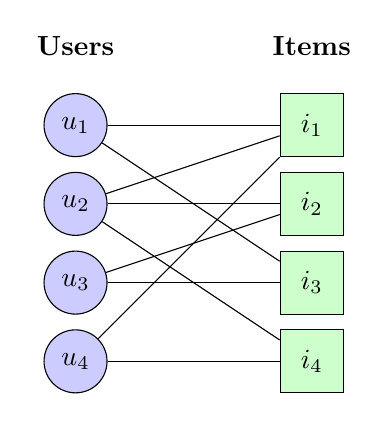
\begin{tikzpicture}[
            user/.style={circle, draw, fill=blue!20, minimum size=0.8cm},
            item/.style={rectangle, draw, fill=green!20, minimum size=0.8cm},
            edge/.style={-}
        ]
        % Users (left side)
        \node[user] (u1) at (0, 3) {$u_1$};
        \node[user] (u2) at (0, 2) {$u_2$};
        \node[user] (u3) at (0, 1) {$u_3$};
        \node[user] (u4) at (0, 0) {$u_4$};
        % Items (right side)
        \node[item] (i1) at (3, 3) {$i_1$};
        \node[item] (i2) at (3, 2) {$i_2$};
        \node[item] (i3) at (3, 1) {$i_3$};
        \node[item] (i4) at (3, 0) {$i_4$};
        % Edges representing user-item interactions
        \draw[edge] (u1) -- (i1);
        \draw[edge] (u1) -- (i3);
        \draw[edge] (u2) -- (i1);
        \draw[edge] (u2) -- (i2);
        \draw[edge] (u2) -- (i4);
        \draw[edge] (u3) -- (i2);
        \draw[edge] (u3) -- (i3);
        \draw[edge] (u4) -- (i1);
        \draw[edge] (u4) -- (i4);
        % Labels
        \node at (0, 4) {\textbf{Users}};
        \node at (3, 4) {\textbf{Items}};
        \end{tikzpicture}
        \subcaption{Bipartite graph representation}
        \label{fig:recommender_graph}
    \end{minipage}%
    \hspace{0.02\textwidth}%
    \begin{minipage}[b]{0.48\textwidth}
        \centering
        \begin{tabular}{|l|c|c|c|c|}
            \hline
            & \textbf{Item 1} & \textbf{Item 2} & \textbf{Item 3} & \textbf{Item 4} \\
            \hline
            User 1 & 4 & 1 & 3 & -- \\
            \hline
            User 2 & 3 & 2 & -- & 4 \\
            \hline
            User 3 & 5 & -- & 2 & 1 \\
            \hline
            User 4 & 2 & 3 & 5 & -- \\
            \hline
        \end{tabular}
        \subcaption{Utility matrix}
        \label{tab:utility_matrix}
    \end{minipage}
    \caption{Recommender system data representation: graph and matrix}
    \label{fig:recommender_combined}
\end{figure}

There are two types of user-item interaction data that can be used for recommendation: \textit{explicit feedback} and \textit{implicit feedback}.

Explicit feedback is feedback where the user consciously expresses their opinion on an item. When a user expresses their opinion on an item by, for example by upvoting or downvoting a social media post, it is a clear indicator of whether the user likes the content or not. This clear signalling makes this type of feedback also generalizable to different domains. An upvote on Reddit means the same thing on all other social media platforms and e-commerce sites. This is probably why explicit feedback is so well researched and understood. 

Even though explicit feedback is well researched and understood, it has a large disadvantage: Users are reluctant to give explicit feedback \parencite{article_implicit_vs_explicit}. It is not always clear why users are reluctant to give feedback, but one of the main reasons is that it requires a bit more effort to give it. Systems that only rely on explicit feedback are not top performing methods because so many user-item interactions are not interpretable if the user does not directly interact with the item. Another disadvantage of explicit feedback is that it can be faked \parencite{lu2012recommender}. For example, on Instagram, it is relatively easy to create bot accounts and like an Instagram picture or inflate follower counts to boost popularity.

Implicit feedback is data collected automatically by observing the behaviour of the user \parencite{article_implicit_vs_explicit}. When the user interacts with the system, for example, information on how long the user has spent looking at an item, is collected. The main advantage of this is that this type of information is abundant. The main disadvantage of implicit feedback is that it is noisy (lot of mixed signals) and requires domain specific interpretation. 

Examples of the challenges in interpreting implicit feedback can be found in multiple domains. One example of the domain specificity is a movie recommendation system tracking watch time. Generally longer watch time means that the movie is more engaging. However, that might not always be the case. What if movie was so boring that the user fell asleep during it? Or what if the user likes to have movies in the background playing when they are home alone? Because of the challenges of interpreting implicit feedback data, more research is required to fully utilize this type of data. It is also less researched because of its domain specific nature and the problems with interpretability.

Explicit and implicit feedback have their own pros and cons. Explicit feedback gives clearer signals of user preference and is easier to interpret. Implicit feedback is very abundant and reflects actual user behaviour and is hard to fake deliberately. The Cons of explicit feedback are data sparsity, prone to bias, and susceptible to manipulation. Implicit feedback suffers from ambiguity, lack of negative signals, and the fact that it requires sophisticated modelling to interpret correctly. \autoref{tab:feedback_characteristics} summarises the characteristics of explicit and implicit feedback.

\begin{table}[h]
\centering
\begin{tabular}{|l|c|c|}
\hline
 & \textbf{Explicit feedback} & \textbf{Implicit feedback} \\
\hline
\textbf{Accuracy} & High & Low \\
\hline
\textbf{Abundance} & Low & High \\
\hline
\textbf{Context-sensitive} & Yes & Yes \\
\hline
\textbf{Expressivity of user preference} & Positive and Negative & Positive \\
\hline
\textbf{Measurement reference} & Absolute & Relative \\
\hline
\end{tabular}
\caption{Summary of the characteristics of explicit feedback characteristics   \parencite{article_implicit_vs_explicit}.}
\label{tab:feedback_characteristics}
\end{table}

\subsection{Challenges in recommender systems}

There are several challenges in recommender systems that decrease the performance of a recommender system. Article \parencite{lu2012recommender} lists eight unique challenges: data sparsity, scalability, cold start, diversity versus accuracy, vulnerability to attacks, time value, recommendation evaluation, and user interface.

\begin{wrapfigure}{r}{0.5\textwidth}
    \centering
    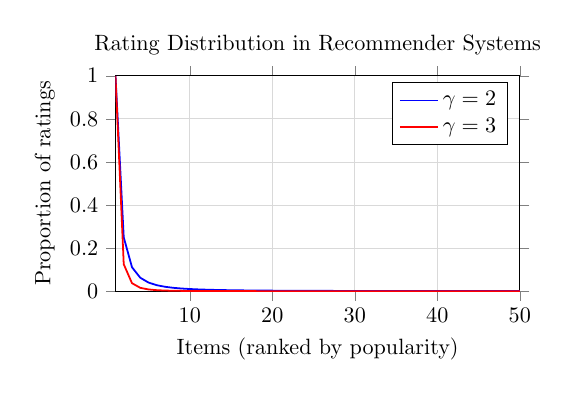
\begin{tikzpicture}[scale=0.8]
        \begin{axis}[
            xlabel={Items (ranked by popularity)},
            ylabel={Proportion of ratings},
            title={Rating Distribution in Recommender Systems},
            xmin=1, xmax=50,
            ymin=0, ymax=1,
            grid=major,
            grid style={gray!30},
            width=8cm,
            height=5cm,
            legend pos=north east,
            tick align=outside,
        ]
        
        % Power law with gamma = 2
        \addplot[
            blue,
            thick,
            domain=1:100,
            samples=100
        ] {x^(-2)};
        \addlegendentry{$\gamma = 2$}
        
        % Power law with gamma = 3
        \addplot[
            red,
            thick,
            domain=1:100,
            samples=100
        ] {x^(-3)};
        \addlegendentry{$\gamma = 3$}
        
        \end{axis}
    \end{tikzpicture}
    \caption{Power law distribution of ratings in recommender systems with $\gamma = 2$ and $\gamma = 3$.}
    \label{fig:power_law}
\end{wrapfigure}

When the data pool is very large in real-world recommender systems, the overlap of two users is often very small or none. This creates a problem called \textit{data sparsity}, where accurate recommendation is difficult due to a lack of data. Furthermore, even when the average number of evaluations per entity is high, it is distributed among the entities unevenly. Typically, the distribution follows a power law, where the form is $P(k) \sim k^{-\gamma}$ with $\gamma$ being a positive exponent usually between 2 and 3 \parencite{RevModPhys.74.47}. As can be seen in \autoref{fig:power_law}, a small minority of items have the majority of ratings. A good recommender system takes this into account because this might cause problems where popular items are suggested more frequently because of the higher representation in the data. 

When new users enter the system, there is no interaction data about them. This hinders the performance of the recommender system and causes inaccurate recommendations for new users. This problem is called the \textit{cold start} problem. The cold start problem is typically tackled with methods that combine multiple recommendation methods. Most of the popular and simple-to-implement solutions perform well enough on users that have a good amount of interaction data. Then there are methods that perform well in the cold start cases. A common approach is to use auxiliary information, such as age, location, or sex of the user. The items can also have auxiliary information about them, such as item name, brand and price.  Another approach is to use data from other sites to make a recommendation on the current site. This can be done by using cookies to save user preferences in the browser.

Most RS use large datasets, so \textit{scalability} is often a bottleneck in implementations. In practice, this can be solved, for example, by computing recommendations from smaller local samples of the data rather than using global data from the whole data set. Another approach is to compute the recommendation incrementally every time new data arrives.

Good recommendation systems are capable of balancing \textit{diversity and precision}. Diversity is the range of different items that are recommended to the user. On a music streaming platform this would mean that the user is recommended songs vastly different from each other from different genres and artists. This helps with new item type discovery, and the user does not get stuck with a single type of music. The reason why balancing between diversity and precision is difficult is because the metrics might counteract each other. Showing the user a wider range of different items might mean that items that the user absolutely like are not shown. 

Another reason why balancing diversity and precision is important is that recommender systems tend to be biased towards popular items. This is because popular items have more connections to users and thus will be recommended more often. Building diversity into the RS also helps with overfitting. With more diverse recommendation, the RS is more generalisable to different domains \parencite{kunaver2017diversity}. 

Recommender systems are \textit{vulnerable to attacks}. An attack on the recommender system can be a malicious actor trying to steal user information, or it can be an attempt to manipulate the algorithm (shilling attack). User data privacy is relatively well secured, with the biggest vulnerabilities being zero-day exploits (vulnerabilities unknown to users), and careless cyber security practises by developers. Manipulation of the RS, on the other hand, is easier. Users can give fake ratings to try to increase or decrease the popularity of an item. The solution to this problem is to identify the attackers quickly and remove fake ratings.

\textit{The interests of users vary over time}. Interests can last from a couple of days to years. An example of this is that a user might be interested in buying a tennis racket from an e-commerce site to go to play with their friends. This interest is a short interest because the user only plays occasionally. On the other hand, they might have a long-term interest in running and buy new shoes every year because the previous shoes are worn. Currently, many recommendation algorithms do not take the decay of interests into account, and it is an ongoing line of research \parencite{lu2012recommender}.

When optimizing an RS, it is important to have \textit{evaluation metrics} for benchmarking the system. The metrics are not absolute and might vary on different datasets. This makes benchmarking recommender systems challenging and makes comparing different recommendation algorithms difficult. In research, the MovieLens datasets are popular for comparing algorithms with each other. In practice, recommender systems have to be tailored to suit the application at hand. There is no universal recommender systems that is able to perform well in all applications. 

A little less technical challenge in RSs is the optimization of the \textit{user interface}. This can be divided into two parts: Firstly, the optimisation of the user interface itself. In the second part, there is the explainability of the recommender system. A common way to display recommendation is with a carousel with the most relevant recommendations being displayed at the top left corner. The further down and right an item is displayed the less likely it is for the user to see it. Explainability is important for the user to trust and use the recommender system more efficiently. Explainability can be implemented by giving reasons why certain items are presented to the user. For example, the used can be shown recommendations in categories like "Because you watched [movie name]" or "Movies directed by [actor name]".


\subsection{Recommender systems performance evaluation}
\label{subsec:performance_evaluation}

When building recommender systems, the goal is to predict unseen ratings as well as possible. To achieve this goal, there is a need to define performance evaluation metrics that quantify the quality of implementations. There are many ways to quantify the quality of a method, and this subsection introduces basics for evaluating RS performance.

There are two notable accuracy metrics for ranking RS accuracy: mean absolute error (MAE) and root mean squared error (RMSE). They are both used to measure the closeness of predicted ratings to real ratings.

MAE and RMSE are defined as 
\[
    \text{MAE} = \frac{1}{|E^P|}\sum_{(i,\alpha)\in E^P}|r_{i\alpha} - \hat{r}_{i\alpha}|
\]

\[
    \text{RMSE} = \left(\frac{1}{|E^P|}\sum_{(i,\alpha)\in E^P}(r_{i\alpha} - \hat{r}_{i\alpha})^2\right)^{\frac{1}{2}}
\]

where $r_{i\alpha}$ is the true rating of object $\alpha$ by user $i$, $\hat{r}_{i\alpha}$ is the predicted rating, and $E^P$ is the set of hidden user-object ratings in the test set. Lower MAE and RMSE correspond to higher prediction accuracy.

In addition to accuracy metrics, there exist other performance metrics. \textit{Classification accuracy metrics} measure the percentage of items that the RS correctly recommended to the user. The \textit{ranking quality metrics} measure the accuracy of the order of recommended items. \textit{Coverage} calculates the proportion of all items that are recommended when recommendations are calculated. A brief summary of popular recommendation metrics can be found in \autoref{tab:recommendation_metrics}.

\begin{table}[h]
\centering
\begin{tabular}{lllccc}
\toprule
Name & Symbol & Preference & Scope & Rank & $L$ \\
\midrule
MAE & $MAE$ & Small & Rating accuracy & No & No \\
RMSE & $RMSE$ & Small & Rating accuracy & No & No \\
Precision & $P(L)$ & Large & Classification accuracy & No & Yes \\
Recall & $R(L)$ & Large & Classification accuracy & No & Yes \\
$F_1$-score & $F_1(L)$ & Large & Classification accuracy & No & Yes \\
AUC & $AUC$ & Large & Classification accuracy & No & No \\
NDCG & $NDCG(L)$ & Large & Ranking quality & Yes & Yes \\
Coverage & $COV(L)$ & Large & Coverage and diversity & No & Yes \\
\bottomrule
\end{tabular}
\caption{A summary of common RS performance metrics. The third column indicates the preference of the metric (e.g. small MAE is better). The last two columns tell whether the method depends on the order of the recommendations and the length of the list of recommendations. Table inspired by article \parencite{lu2012recommender}.}
\label{tab:recommendation_metrics}
\end{table}

To benchmark a recommender system, a dataset of ratings is needed. Luckily, there exists multiple high quality open source datasets for benchmarking. The MovieLens data set is one of the most widely used data set in research. The data is gathered from the MovieLens web site and is maintained by a research lab GroupLens from the University of Minnesota. Different versions of the dataset can be found from \url{https://grouplens.org/datasets/movielens/} containing different amounts of ratings, synthetized ratings and datasets with varying time intervals for when they were collected. MovieLens is one of the more popular open source datasets for benchmarking recommender systems, but there are other great ones out there. The GitHub page, \parencite{costa2024datasets}, has great links other great datasets for benchmarking recommender systems.


\subsection{Lessons from the 2006 Netflix prize}

In 2006, Netflix organised a recommender system competition. The goal of the competition was to improve their current recommender system, Cinematch. For the competition, Netflix released a dataset containing 100 million anonymous movie ratings. The winning solution was required to improve the RMSE of Cinematch by 10\%. The prize for the winner was one million dollars so the stakes were high.

The competition attracted international intrest and over 20 thousand teams signed up from 152 different countries. Despite the massive amount of participants, only 90 teams were able to improve the accuracy by more than 5\%. After three years of intense competition, the 10\% goal set by Netflix was reached on September 18, 2009, when the team BellKor's Pragmatic Chaos was declared the winner.

The first-year winner BellKor wrote a popular research article on their findings \parencite{bell2007lessons}. In the article, the importance of utilising a variety of models is emphasised. In other words, \textit{a complete recommender system should use a combination of different algorithms to combine the strengths of the models}. The best way to choose algorithms to be combined was to use methods that utilise different aspects of the data. This way the system does not have blind spots and is able to create better recommendations.

BellKor's first year winning solution was a weighted linear method where they combined all methods they had researched. The solution used 107 different algorithms, but they stated that the amount of algorithms was unnecessarily large. In their article \parencite{bell2007lessons}, they mention that the amount was that large because of algorithms being added to the system every time one was researched and tested. The paper published by the 2009 winning team were able to use only 18 algorithms to achieve the 10\% prediction improvement required by Netflix to win the grand prize \parencite{toscher2009bigchaos}. 


\newpage

\section{Traditional recommender systems}
\label{sec:traditional_RS}

Traditional recommender systems are typically classified into content-based, collaborative, and hybrid filtering. \textit{Content-based filtering} creates recommendations based on items similar to those that the user preferred in the past. In \textit{collaborative filtering} the user is recommended items that people with similar tastes and preferences like. Lastly, \textit{hybrid methods} combine the strengths of collaborative, content-based filtering, and other methods to create more powerful recommender systems. The taxonomy is visualised in \autoref{fig:RS_taxonomy}.

\begin{figure}[h]
\centering
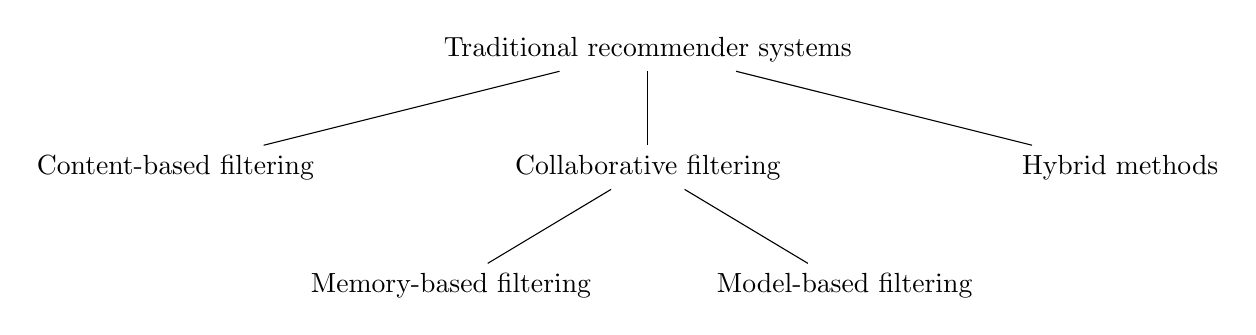
\begin{tikzpicture}[level distance=1.5cm, sibling distance=2.5cm]
\tikzset{
    every node/.style={align=center},
    level 1/.style={sibling distance=6cm},
    level 2/.style={sibling distance=5cm}
}

\node {Traditional recommender systems}
    child {
        node {Content-based filtering}
    }
    child {
        node {Collaborative filtering}
        child {
            node {Memory-based filtering}
        }
        child {
            node {Model-based filtering}
        }
    }
    child {
        node {Hybrid methods}
    };
\end{tikzpicture}

\caption{Types of recommender systems}
\label{fig:RS_taxonomy}
\end{figure}

\subsection{Content-based filtering}
\label{subsec:content_based_filtering}

\begin{figure}[h]
\centering
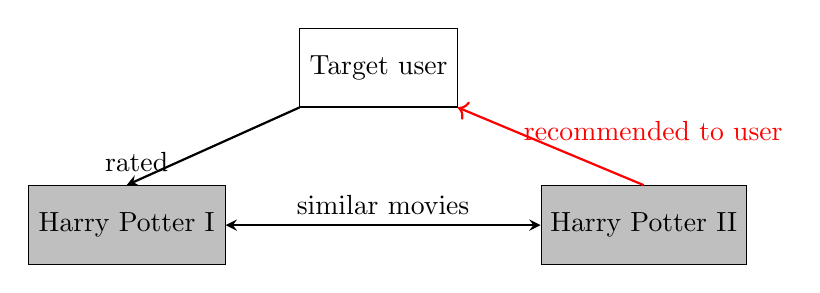
\begin{tikzpicture}[
    node distance=3cm,
    every node/.style={align=center},
    user/.style={draw, rectangle, fill=white, minimum width=2cm, minimum height=1cm},
    movie/.style={draw, rectangle, fill=gray!50, minimum width=2.5cm, minimum height=1cm},
    arrow/.style={->, thick, >=stealth},
    redarrow/.style={->, thick, red},
]
% Target user at the top
\node[user] (target) at (3.2,2) {Target user};
% Movies at the bottom
\node[movie] (hp1) at (0,0) {Harry Potter I};
\node[movie, right=4cm of hp1] (hp2) {Harry Potter II};
% Arrows
\draw[arrow] (target.south west) -- node[left, pos=0.7] {rated} (hp1.north);
\draw[<->, thick, >=stealth] (hp1.east) -- node[above] {similar movies} (hp2.west);
\draw[redarrow] (hp2.north) -- node[right, pos=0.7] {recommended to user} (target.south east);
\end{tikzpicture}
\caption{Content-based filtering. The main assumption is that users like similar items that they have liked in the past. Similar items are determined by item attributes.}
\label{fig:content_based_filtering1}
\end{figure}

Content-based filtering assumes that users are interested in similar items that they have liked in the past \parencite{al2024traditional}. This is done by first extracting the information of the item to be recommended. Then the item information is compared to items the user has previously liked. If the item is similar to items the user has previously liked, the item is recommended. 

\subsection{Collaborative Filtering}
\label{subsec:collaborative_filtering}

The main technique behind collaborative filtering is that item and user similarity is calculated by the collaborative ratings of items \parencite{al2024traditional}. This is why the technique is called collaborative filtering. In short, similar users are found by comparing their rating histories and similar items are found by comparing ratings from users. The way user ratings are used, can be further divided into two classes: \textit{memory-based} and \textit{model-based} techniques. Memory-based CF learns the the similarity of users or items from rating data, and then recommendations are made based on similarity data. Model-based CF uses machine learning models to predict rating data. Memory-based filtering can be further classified into \textit{user-based} and \textit{item-based} filtering based on if the filtering is based on user or item similarity. 

\subsubsection{Memory-based collaborative filtering}
\label{subsubsec:memory_based_filtering}

\begin{figure}[h]
\centering
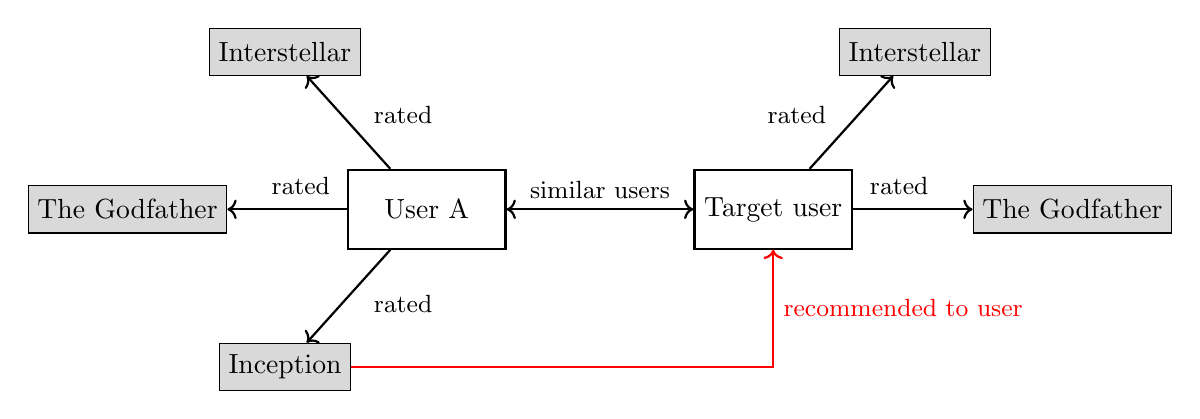
\begin{tikzpicture}[
    node distance=2cm,
    film/.style={circle, draw, minimum size=0.8cm, thick},
    user/.style={rectangle, draw, minimum width=2cm, minimum height=1cm, thick},
    movie/.style={rectangle, draw, minimum width=1.5cm, minimum height=0.6cm, fill=gray!30},
    arrow/.style={->, thick},
    redarrow/.style={->, thick, red},
    doublearrow/.style={<->, thick},
    label/.style={font=\small}
]
% Define positions
\coordinate (center) at (0,0);
% Users
\node[user] (userA) at (-2.2,0) {User A};
\node[user] (target) at (2.2,0) {Target user};
% Movies for User A (left side)
\node[movie] (int1) at (-4,2) {Interstellar};
\node[movie] (god1) at (-6,0) {The Godfather};
\node[movie] (inc1) at (-4,-2) {Inception};
% Movies for Target user (right side)
\node[movie] (int2) at (4,2) {Interstellar};
\node[movie] (god2) at (6,-0) {The Godfather};

% Arrows from movies to users
\draw[arrow] (userA) -- (int1);
\node[label] at (-2.5, 1.2) {rated};

\draw[arrow] (userA) -- (god1);
\node[label] at (-3.8, 0.3) {rated};

\draw[arrow] (userA) -- (inc1);
\node[label] at (-2.5, -1.2) {rated};

\draw[arrow] (target) -- (int2);
\node[label] at (2.5, 1.2) {rated};

\draw[arrow] (target) -- (god2);
\node[label] at (3.8, 0.3) {rated};

% Similar user connection
\draw[doublearrow] (userA) -- (target) node[midway, above, label] {similar users};
% Recommendation arrow
\draw[redarrow] (inc1) -- (2.2, -2) -- (target) node[midway, right, label] {recommended to user};
\end{tikzpicture}
\caption{User-based collaborative filtering. Similar users have similar rating histories.}
\label{fig:collaborative_filtering}
\end{figure}

\textit{User-based CF} uses user similarity to predict ratings. To do this, users are first modelled as vectors based on their rating profiles. Their rating vector will consist of all the ratings they have given to each item. Then these user vectors are compared with a vector similarity metric. Then the $k$ nearest neighbours (the $k$ most similar users) are computed. Then, all the items rated by the nearest neighbours are aggregated into one set and the items rated by the target user are removed. Then, the most frequent items in the set are recommended to the user sorted in decreasing order based on item frequency.

\begin{figure}[h]
\centering
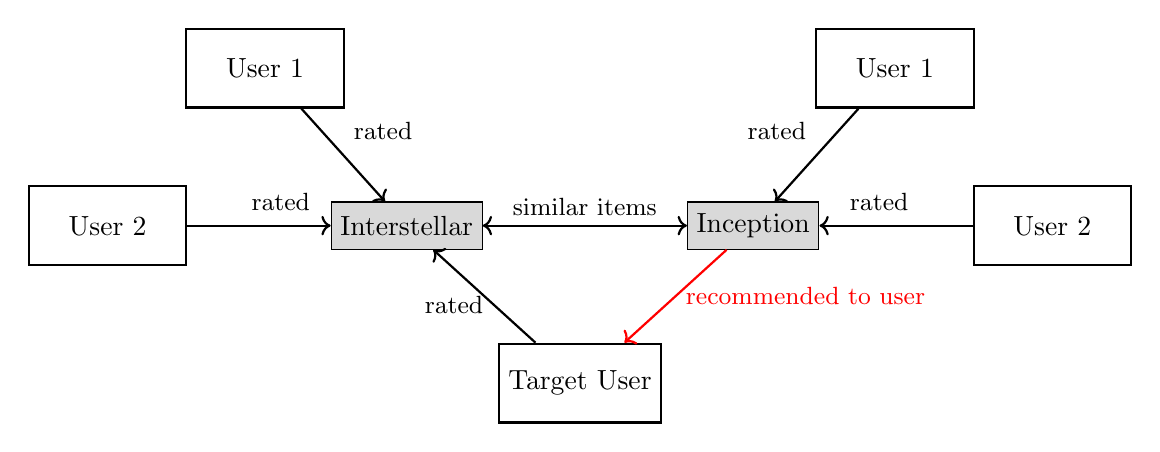
\begin{tikzpicture}[
    node distance=2cm,
    film/.style={circle, draw, minimum size=0.8cm, thick},
    user/.style={rectangle, draw, minimum width=2cm, minimum height=1cm, thick},
    movie/.style={rectangle, draw, minimum width=1.5cm, minimum height=0.6cm, fill=gray!30},
    arrow/.style={->, thick},
    redarrow/.style={->, thick, red},
    doublearrow/.style={<->, thick},
    label/.style={font=\small}
]

% Define positions
\coordinate (center) at (0,0);

% Target item and similar item
\node[movie] (similar_item) at (-2.2,0) {Interstellar};
\node[movie] (target_item) at (2.2,0) {Inception};

% Users for target item (left side)
\node[user] (user1) at (-4,2) {User 1};
\node[user] (user2) at (-6,0) {User 2};

% Users for similar item (right side)
\node[user] (user1b) at (4,2) {User 1};
\node[user] (user2b) at (6,0) {User 2};
\node[user] (target_user) at (0,-2) {Target User};

% Arrows from users to movies
\draw[arrow] (user1) -- (similar_item);
\node[label] at (-2.5, 1.2) {rated};

\draw[arrow] (user2) -- (similar_item);
\node[label] at (-3.8, 0.3) {rated};

\draw[arrow] (user1b) -- (target_item);
\node[label] at (2.5, 1.2) {rated};

\draw[arrow] (user2b) -- (target_item);
\node[label] at (3.8, 0.3) {rated};

\draw[arrow] (target_user) -- (similar_item);
\node[label] at (-1.6, -1) {rated};

% Similar items connection
\draw[doublearrow] (target_item) -- (similar_item) node[midway, above, label] {similar items};

% Recommendation arrow
\draw[redarrow] (target_item) -- (target_user) node[midway, right, label] {recommended to user};

\end{tikzpicture}
\caption{Item-based collaborative filtering. Similar items have similar ratings from the same users.}
\label{fig:item_based_collaborative_filtering}
\end{figure}

\textit{Item-based CF} uses item similarity to predict ratings. The difference with user-based CF is that items are now represented as vectors, where the vector contains all the ratings the item has received. Then similarly to user-based CF, item similarity is calculated between the item vectors. The items most similar to the items the user has rated will then be recommended to the user, sorted in a decreasing order by item similarity.

In memory-based CF, an example of a similarity metric is cosine-based similarity \parencite{su2009survey}. Cosine-based similarity is defined as the normalized dot product of two vectors, $\text{sim}(\mathbf{A}, \mathbf{B}) = \frac{\mathbf{A} \cdot \mathbf{B}}{||\mathbf{A}||_2 \, ||\mathbf{B}||_2}$, and tells how similar the directions of the vectors are. With cosine-based similarity a high positive number indicates high similarity, a high negative value indicates opposites and zero is neutral.

\subsubsection{Model-based collaborative filtering}
\label{subsubsec:model_based_filtering}

The name model-based CF comes from the fact that machine learning models are used to predict ratings. Machine learning methods excel in this task because they are great at predicting non-linear relationships in the user-item interaction data. The main advantages of model-based filtering methods are that after training, they require less memory and compute than other methods. Commonly used models include Bayesian models, clustering models, and dependency networks. From these algorithms, classification algorithms can be used as CF models if user ratings are categorical, and regression models and SVD methods can be used for numerical ratings \parencite{su2009survey}.

\subsection{Hybrid methods}
\label{subsec:hybrid_method}

Hybrid methods combine the strengths of different methods to create even more powerful methods. The best combination is achieved by combining methods that address different aspects of the data \parencite{bell2007lessons}. A common example of a hybrid method is weighted hybridization. In this hybrid method, different recommendation algorithms are given importance scores (weights) based on their ability to predict correct ratings. Then the outputs of all recommendation algorithms are weighted based on predefined weights and combined to create recommendations. More popular hybrid methods can be found from \autoref{tab:hybrid_methods}.

\begin{table}[h]
\centering
\begin{tabular}{p{4cm}p{8cm}}
\toprule
\textbf{Method name} & \textbf{Description} \\
\midrule
Weighted hybridization & The output of different recommender systems are weighted based on their ability predict ratings. Then the weighted results are combined and shown to the user. \\
Switching hybridization & Recommender systems are switched based on the recommendation scenario. \\
Mixed hybridization & Multiple recommender systems calculate recommendations. Then the outputs of these systems are mixed and shown to the user. \\
Cascade hybridization & A primary system creates a list of recommendations. Then a secondary system tweaks the recommendations typically addressing a problem in the primary system. \\
Feature combination & A secondary RS calculates feature vectors for users or items and enhances the primary system with these features. \\
Feature augmentation & User or item feature vectors are used as input for another recommender system. \\
Meta-level & A system replaces the original dataset with augmented data and another then creates recommendations based on this data. \\
\bottomrule
\end{tabular}
\caption{Popular hybrid methods \parencite{roy2022systematic}.}
\label{tab:hybrid_methods}
\end{table}

\subsection{Advantages and Limitations of traditional recommender systems}

Traditional methods have become popular because they are easy to implement and perform well enough for most applications. This is why traditional methods typically serve as a baseline in industry. Although traditional methods are widely used in industry, it is important to understand in which scenarios traditional methods perform well, and in which scenario they tend to struggle. This way appropriate methods can be chosen for each application.

\subsubsection{Content-based filtering}

The main \textit{advantages} of content-based filtering are good performance with sparse interaction data (immunity to the cold-start problem) \parencite{al2024traditional} and the explainability of recommendations. CBF performs well with sparse data because the method relies only on item attribute data. Of course, the user has to first interact with a few items but then the  algorithm is able to recommend similar items based on item profiles. Because CBF uses item similarity to create recommendations, the methods are more explainable. For example, an e-commerce site could have a category of "similar products to [product]". 

There are three main \textit{disadvantages} of content-based filtering: limited discovery, feature engineering, and the cold-start problem for items. Because recommendations are based only on the features of items, CBF has a hard time discovering new items \parencite{al2024traditional}. The algorithm will only recommend items similar to items that have been previously liked. The second disadvantage, feature engineering, means that it is difficult to decide the item attributes recommendations should be based on. Often processing these features can also be challenging (e.g. image/video processing). The third weakness is that if an item has little or no information about it, the item will not be recommended to the user. 

\subsubsection{Collaborative filtering}

The main \textit{advantages} of collaborative filtering is its ability to capture complex user preferences and adapt to changing user tastes \parencite{al2024traditional}. This is because recommendation is based on user-item interaction data. A side effect of recommendation being based on interaction data is that CF recommender systems generalize well to multiple domains.

\textit{Disadvantages} of collaborative filtering are reduced performance on sparse data and scalability issues \parencite{jetti2025knowledge}. Because the recommendation is based on user-item interaction data, users with little to no interaction data struggle to get good recommendations. Data sparsity issues also arise in large item catalogues with many items. In this case, the user-item matrix becomes sparse, leading to difficulties computing similarities due to data sparsity. Scalability issues arise from high computational costs when dealing with large-scale datasets. Because CF uses large amounts of user-item interaction data to calculate similarities, computational costs increase with the amount of data. 

\subsubsection{Hybrid methods}

Hybrid methods typically \textit{perform better} than CF and CBF methods because they combine the strengths of multiple different methods. In this way, disadvantages such as data sparsity issues can be mitigated by adding methods to the system that do not suffer from data sparsity. Hybrid methods also provide flexibility when designing a recommendation system for specific applications. RSs can be optimised to perform ideally in specific applications. 

The increased complexity is, on the other hand, is a \textit{disadvantage} of hybrid methods. Increased complexity makes maintaining the system more difficult and also increases computational costs. Perfecting hybrid methods also requires a lot of tuning and optimizing to achieve the optimal performance, and this takes a lot of time, effort and skill \parencite{al2024traditional}.

\newpage

\section{Knowledge graphs}
\label{sec:knowledge_graphs}

Knowledge graphs are added to recommender systems to add auxiliary data to help with recommendation. The concept of knowledge graphs was developed in the 1980s when KGs were integrated into expert systems in medical and social sciences \parencite{nurdiati200825}. Back then, knowledge graphs were simpler consisting of fewer entity and relation types. In 2012 Google broadened the concept to the linguistic and logical domains. At Google, they successfully applied KGs in their web search system. 

After Google popularised knowledge graphs, KGs have gained attention in applications that need to exploit diverse, dynamic, and large-scale collections of data. KGs are a great tool for these applications because they can store semantic information. Another benefit of KGs is that KGs can help postpone the definition of a data schema. This means that the data can evolve more flexibly \parencite{10.1145/3104031}. 

There is no widely agreed-upon definition of a knowledge graph. Generally, a knowledge graph can be described as a heterogeneous information network (contains multiple types of entities and relations). A heterogeneous information network (HIN) is a rigorously defined concept and often functions as a baseline when defining KGs. HINs can be defined as in article \parencite{guo2020survey}:

\begin{definition}[Heterogeneous information network]
\label{def:HIN}
A heterogeneous information network is a directed graph $G = (V,E)$ with an entity-type mapping function $\phi : V \rightarrow \mathcal{A}$ and a relation-type mapping function $\psi: E \rightarrow \mathcal{R}$. Each entity $v\in V$ belongs to an entity type $\phi(v) \in \mathcal{A}$, and each relation $e\in E$ belongs to a relation type $\psi(e) \in \mathcal{R}$. In addition, the number of entity types $|\mathcal{A|}>1$ and/or the number of relation types is $|\mathcal{R}|>1$.
\end{definition}

\begin{figure}[h]
    \centering
    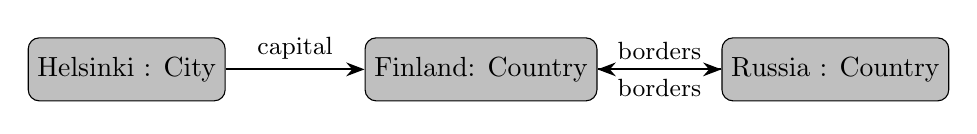
\begin{tikzpicture}[
        node distance=2cm,
        widebox/.style={draw, rounded corners, minimum width=2.5cm, minimum height=0.8cm, align=center, fill=lightgray},
        arrow/.style={->, >=Stealth, thick},
        black_arrow/.style={arrow, color=black},
        black_label/.style={color=black, font=\small}
    ]
    % Heterogeneous graph nodes with type labels
    \node[widebox] (santiago_city) at (-1.5, 0) {Helsinki : City};
    \node[widebox] (chile_country) at (3, 0) {Finland: Country};
    \node[widebox] (peru_country) at (7.5, 0) {Russia : Country};
    
    % Arrows and labels for Heterogeneous graph
    \draw[black_arrow] (santiago_city) -- (chile_country) node[midway, above, black_label] {capital};
    \draw[black_arrow] (chile_country) -- (peru_country) node[midway, above, black_label] {borders};
    \draw[black_arrow] (peru_country) -- (chile_country) node[midway, below, black_label] {borders};
    \end{tikzpicture}
    \caption{Heterogeneous information graph representation. Inspired by \parencite{hogan2021knowledge}}
    \label{fig:heterogeneous_graph}
\end{figure}

The main difference between HINs and KGs is the scale and diversity of the types of nodes and entities \parencite{sun2022heterogeneous}. Most HINs have relatively simple schemas, which means that the graphs have a small number of types of entities and relations. On the other hand, KGs have a much richer network schema, with hundreds or even thousands of entity and relation types. The paths in the graph create facts such as $Helsinki \xrightarrow{capital\ of}Finland \xrightarrow{next\ to}Russia$. These paths store complex connections and help reason facts such as the fact that the city Helsinki is near Russia. An example of a knowledge graph can be found in \autoref{fig:movie_kg}.

This thesis uses the following definition for knowledge graphs from article \parencite{Ji_2022}: 

\begin{definition}[Knowledge graph]
\label{def:KG_formal}
A knowledge graph is a directed graph $\mathcal{G = \{\mathcal{E}, \mathcal{R}, \mathcal{F}\}}$, where $\mathcal{E}$, $\mathcal{R}$ and $\mathcal{F}$ are the sets of entities, relations and facts. A fact $f$ is denoted as a triple $(h,r,t)$, where $h \in \mathcal{E}$, $r \in \mathcal{R}$ and $t\in \mathcal{E}$ are the head entity, relation, and tail entity of a fact $f \in\mathcal{F}$.
\end{definition}

\begin{figure}[h]
\centering
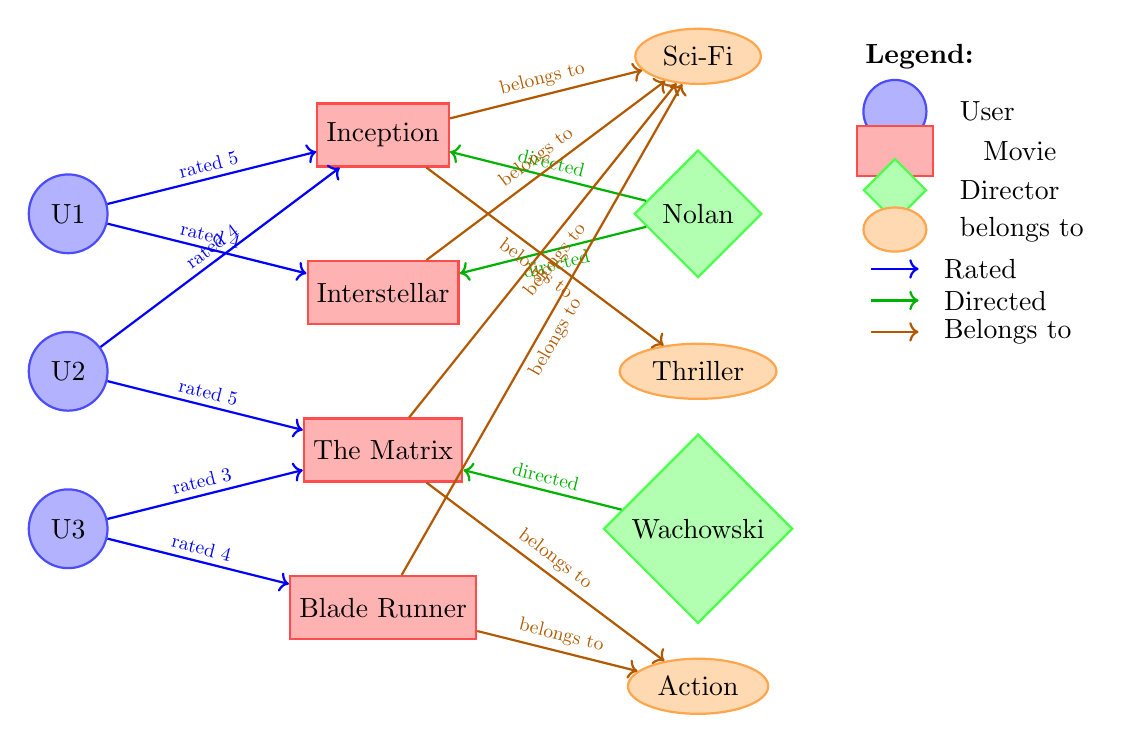
\begin{tikzpicture}[
    % Node styles
    user/.style={circle, fill=blue!30, draw=blue!70, thick, minimum size=1cm},
    movie/.style={rectangle, fill=red!30, draw=red!70, thick, minimum width=1.2cm, minimum height=0.8cm},
    director/.style={diamond, fill=green!30, draw=green!70, thick, minimum size=1cm},
    belongs to/.style={ellipse, fill=orange!30, draw=orange!70, thick, minimum width=1cm, minimum height=0.7cm},
    % Edge styles
    rated/.style={->, thick, blue},
    directed/.style={->, thick, green!70!black},
    belongs/.style={->, thick, orange!70!black}
]
% User nodes
\node[user] (u1) at (0, 4) {U1};
\node[user] (u2) at (0, 2) {U2};
\node[user] (u3) at (0, 0) {U3};
% Movie nodes
\node[movie] (m1) at (4, 5) {Inception};
\node[movie] (m2) at (4, 3) {Interstellar};
\node[movie] (m3) at (4, 1) {The Matrix};
\node[movie] (m4) at (4, -1) {Blade Runner};
% Director nodes
\node[director] (d1) at (8, 4) {Nolan};
\node[director] (d2) at (8, 0) {Wachowski};
% belongs to nodes
\node[belongs to] (g1) at (8, 6) {Sci-Fi};
\node[belongs to] (g2) at (8, 2) {Thriller};
\node[belongs to] (g3) at (8, -2) {Action};
% User-Movie relationships (ratings)
\draw[rated] (u1) -- (m1) node[midway, above, sloped, scale=0.7] {rated 5};
\draw[rated] (u1) -- (m2) node[midway, above, sloped, scale=0.7] {rated 4};
\draw[rated] (u2) -- (m1) node[midway, above, sloped, scale=0.7] {rated 4};
\draw[rated] (u2) -- (m3) node[midway, above, sloped, scale=0.7] {rated 5};
\draw[rated] (u3) -- (m3) node[midway, above, sloped, scale=0.7] {rated 3};
\draw[rated] (u3) -- (m4) node[midway, above, sloped, scale=0.7] {rated 4};
% Director-Movie relationships
\draw[directed] (d1) -- (m1) node[midway, above, sloped, scale=0.7] {directed};
\draw[directed] (d1) -- (m2) node[midway, below, sloped, scale=0.7] {directed};
\draw[directed] (d2) -- (m3) node[midway, above, sloped, scale=0.7] {directed};
% Movie-genre relationships
\draw[belongs] (m1) -- (g1) node[midway, above, sloped, scale=0.7] {belongs to};
\draw[belongs] (m1) -- (g2) node[midway, below, sloped, scale=0.7] {belongs to};
\draw[belongs] (m2) -- (g1) node[midway, above, sloped, scale=0.7] {belongs to};
\draw[belongs] (m3) -- (g1) node[midway, below, sloped, scale=0.7] {belongs to};
\draw[belongs] (m3) -- (g3) node[midway, above, sloped, scale=0.7] {belongs to};
\draw[belongs] (m4) -- (g1) node[midway, below, sloped, scale=0.7] {belongs to};
\draw[belongs] (m4) -- (g3) node[midway, above, sloped, scale=0.7] {belongs to};
% Legend
\node[anchor=west] at (10, 6) {\textbf{Legend:}};
\node[user, scale=0.8] at (10.5, 5.3) {};
\node[anchor=west] at (11.2, 5.3) {User};
\node[movie, scale=0.8] at (10.5, 4.8) {};
\node[anchor=west] at (11.5, 4.8) {Movie};
\node[director, scale=0.8] at (10.5, 4.3) {};
\node[anchor=west] at (11.2, 4.3) {Director};
\node[belongs to, scale=0.8] at (10.5, 3.8) {};
\node[anchor=west] at (11.2, 3.8) {belongs to};
\draw[rated] (10.2, 3.3) -- (10.8, 3.3);
\node[anchor=west] at (11, 3.3) {Rated};
\draw[directed] (10.2, 2.9) -- (10.8, 2.9);
\node[anchor=west] at (11, 2.9) {Directed};
\draw[belongs] (10.2, 2.5) -- (10.8, 2.5);
\node[anchor=west] at (11, 2.5) {Belongs to};
\end{tikzpicture}
\caption{Knowledge graph for movie recommendation. The graph shows relationships between users (circles), movies (rectangles), directors (diamonds), and genres (ellipses).}
\label{fig:movie_kg}
\end{figure}

\newpage

\section{Knowledge graph modelling methods}
\label{sec:knowledge_graph_modelling}


The methods for modelling knowledge graphs in RSs to are divided into three categories: \textit{path-based}, \textit{embedding-based} and \textit{unified} methods (see \autoref{fig:KG_topic_tree}). Path-based methods use graph algorithms to directly explore the graph and find connection patterns between users and items. Embedding-based methods embed the graph to a low-dimensional space so that machine learning methods can be used. Lastly, unified methods combine path-based and embedding-based techniques to combine the strengths of both methods. Most unified methods involve deep learning and graph neural networks.

\begin{figure}[h]
\centering
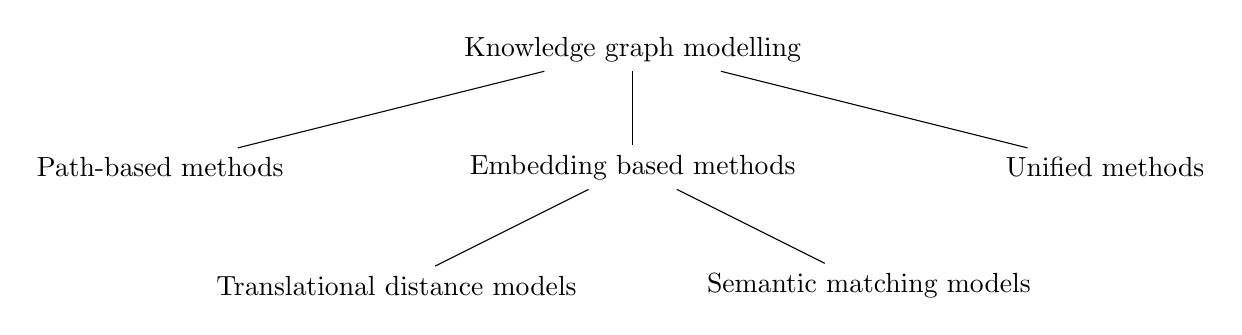
\begin{tikzpicture}[level distance=1.5cm, sibling distance=2.5cm]
\tikzset{
    every node/.style={align=center},
    level 1/.style={sibling distance=6cm},
    level 2/.style={sibling distance=6cm}
}

\node {Knowledge graph modelling}
    child {
        node {Path-based methods}
    }
    child {
        node {Embedding based methods}
        child {
            node {Translational distance models}
        }
        child {
            node {Semantic matching models}
        }
    }
    child {
        node {Unified methods}
    };
\end{tikzpicture}

\caption{Knowledge graph taxonomy.}
\label{fig:KG_topic_tree}
\end{figure}

\subsection{Path-based Methods}
\label{subsec:path_based_methods}

Path-based methods use connective patterns in the knowledge graph to create recommendations. These connective patterns are analysed with different graph analysis algorithms. These connective patterns are called \textit{meta-paths} and are defined in \parencite{guo2020survey} as the following:

\begin{definition}[Meta-path]
\label{def:meta_path}
    Let a graph be defined as $\mathcal{G} = \{\mathcal{E}, \mathcal{R}\}$, where $e_i \in \mathcal{E}$ represents an entity (node) in the set of all entities (nodes) and $r_i \in \mathcal{R}$ represents a relation in the set of all relations. Then a \textbf{meta-path} $\mathcal{P} = e_0 \xrightarrow{r_1} e_1 \xrightarrow{r_2} \ldots \xrightarrow{r_k} e_k$ is a path between entities $e_0$ and $e_k$ defined in the graph $\mathcal{G}$.
\end{definition}

Meta-paths can be used to calculate entity similarity. Similarity metrics are useful for recommendation because recommendation can then be done in a similar manner than in traditional methods; Two similar users will probably enjoy similar items and a user will enjoy similar items to the items they have enjoyed in the past. The most common metric for calculating entity similarity in a graph is a method called $PathSim$ introduced by \textcite{sun2011pathsim} in \citeyear{sun2011pathsim}:

\begin{definition}[PathSim]
\label{def:pathsim}
    Let $p_{e_i \leadsto e_j}$ be a path between entities $e_i$ and $e_j$ and $\mathcal{P}$ a symmetric path (a path that is the same traversed in both directions). Then the path-based similarity score is
    \[
        s_{x,y} = \frac{2 \times |\{p_{x \leadsto y} : p_{x \leadsto y} \in \mathcal{P}\}|}{|\{p_{x \leadsto x} : p_{x \leadsto x} \in \mathcal{P}\}| + |\{p_{y \leadsto y} : p_{y \leadsto y} \in \mathcal{P}\}|}
    \]
\end{definition}

PathSim can be applied to create latent representations of users and items. The similarity score can be used to force the latent representations close to each other by using a norm. When the similarity score is multiplied by the difference of the latent representation, the difference is minimized. This concept is formally written in \parencite{guo2020survey} as:

\begin{definition}[Entity similarity] 
\label{def:entity_similarity}

With $||\cdot||_F$ denoting the matrix Forbenious norm, $\Theta = [\theta_1, \theta_2, \ldots,  \theta_L]$ denoting the weights of each meta path and $\mathbf{U} = [\mathbf{u}_1, \mathbf{u}_2, \ldots, \mathbf{u}_m]$ denoting latent vectors of all users, $s^l_{i,j}$ denoting the similarity score \eqref{def:pathsim} of users i and j on meta-path l and $\mathbf{V} = [\mathbf{v_1}, \mathbf{v_2}, \ldots, \mathbf{v_n}]$ denoting the latent vectors of all items, the similarity scores between entities are:

\textbf{User-User similarity}

\[
    \min_{U,\Theta} \sum_{l=1}^{L} \theta_l \sum_{i=1}^{m} \sum_{j=1}^{m} s_{i,j}^l \|\mathbf{u}_i - \mathbf{u}_j\|_F^2
\]

\textbf{Item-Item similarity}

\[
    \min_{V,\Theta} \sum_{l=1}^{L} \theta_l \sum_{i=1}^{n} \sum_{j=1}^{n} s_{i,j}^l \|\mathbf{v}_i - \mathbf{v}_j\|_F^2
\]

\textbf{User-Item similarity}

\[
    \min_{U,V,\Theta} \sum_{l=1}^{L} \theta_l \sum_{i=1}^{m} \sum_{j=1}^{n} (\mathbf{u}_i^T \mathbf{v}_j - s_{i,j}^l)^2
\]
\end{definition}


\subsection{Embedding-based methods}
\label{subsec:embedding_based_methods}

Embedding-based methods encode the structural information of a KG into a low-dimensional vector space. When computing an embedding, the process can be divided into two steps. The first step is defining a scoring/loss function $f_r(h,t)$, where $h$ is a head entity, $t$ is a tail entity and $r$ is the relation between the head and tail entity. The second step is to minimize the loss function $f_r(h,t)$. The vector embedding that minimizes the loss function preserves as much structural information as possible. 

After the loss function is minimized, it can be used in reverse to determine true relations from false ones. If the loss function is small for a triple $(h,r,t)$, the triple is more likely to be a true triple of the original KG. If the loss function is large for a triple, the triple is likely to be false. Using this logic, the knowledge graph can be reconstructed again from the embedding using the loss function by setting a decision boundary for true and false triples.

Embedding-based methods can be divided into two classes based on how the loss function models the correctness of a triple: \textit{translation distance models} and \textit{semantic matching models}.

\begin{figure}[h]
\centering
% TransE diagram
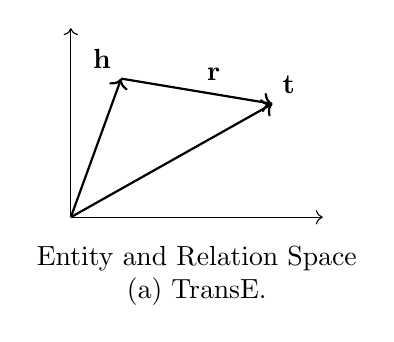
\begin{tikzpicture}[scale=0.8]
\label{subfig:transE}
    % Coordinate system
    \draw[->] (0,0) -- (4,0);
    \draw[->] (0,0) -- (0,3);
    
    % Points
    \coordinate (O) at (0,0);
    \coordinate (h) at (0.8,2.2);
    \coordinate (t) at (3.2,1.8);
    \coordinate (r_start) at (4.8,3);
    
    % Vectors
    \draw[->, thick] (O) -- (h) node[above left] {$\mathbf{h}$};
    \draw[->, thick] (O) -- (t) node[above right] {$\mathbf{t}$};
    \draw[->, thick] (h) -- (t) node[midway, above right] {$\mathbf{r}$};
    
    % Labels
    \node[below] at (2,-0.3) {Entity and Relation Space};
    \node[below] at (2,-0.8) {(a) TransE.};
\end{tikzpicture}
\hspace{1cm}
% TransH diagram
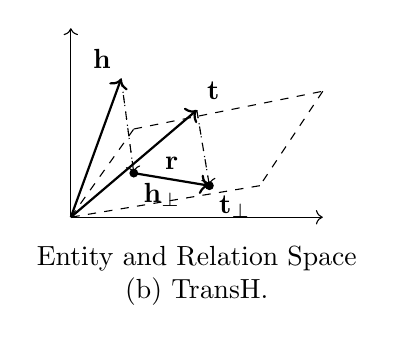
\begin{tikzpicture}[scale=0.8]
\label{subfig:transH}
    % Coordinate system
    \draw[->] (0,0) -- (4,0);
    \draw[->] (0,0) -- (0,3);
    % Hyperplane coords
    \coordinate (h1) at (0,0);
    \coordinate (h2) at (1,1.4);
    \coordinate (h3) at (4,2);
    \coordinate (h4) at (3,0.5);
    
    % Hyperplane (dashed line)
    \draw[dashed] (h1) -- (h2);
    \draw[dashed] (h2) -- (h3);
    \draw[dashed] (h3) -- (h4);
    \draw[dashed] (h4) -- (h1);
    
    % Points
    \coordinate (O) at (0,0);
    \coordinate (h) at (0.8,2.2);
    \coordinate (t) at (2,1.7);
    \coordinate (h_proj) at (1,0.7);
    \coordinate (t_proj) at (2.2,0.5);
    
    % Original vectors
    \draw[->, thick] (O) -- (h) node[above left] {$\mathbf{h}$};
    \draw[->, thick] (O) -- (t) node[above right] {$\mathbf{t}$};
    % Relation vector
    \draw[->, thick] (h_proj) -- (t_proj) node[midway, above] {$\mathbf{r}$};
    
    % Projected vectors
    \draw[->, dashed] (h) -- (h_proj) node[below right] {$\mathbf{h}_{\perp}$};
    \draw[->, dashed] (t) -- (t_proj) node[below right] {$\mathbf{t}_{\perp}$};
    
    % Projection lines
    \draw[dotted] (h) -- (h_proj);
    \draw[dotted] (t) -- (t_proj);
    % Points at projections
    \fill (h_proj) circle (2pt);
    \fill (t_proj) circle (2pt);
    
    % Labels
    \node[below] at (2,-0.3) {Entity and Relation Space};
    \node[below] at (2,-0.8) {(b) TransH.};
\end{tikzpicture}
\vspace{0.5cm}
% TransR diagram - Combined Entity and Relation Space
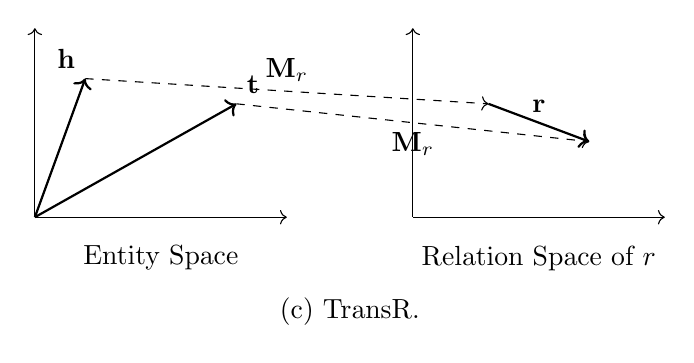
\begin{tikzpicture}[scale=0.8]
\label{subfig:transR}
    % Entity Space (left side)
    % Coordinate system
    \draw[->] (0,0) -- (4,0);
    \draw[->] (0,0) -- (0,3);
    
    % Points in entity space
    \coordinate (O1) at (0,0);
    \coordinate (h) at (0.8,2.2);
    \coordinate (t) at (3.2,1.8);
    
    % Vectors in entity space
    \draw[->, thick] (O1) -- (h) node[above left] {$\mathbf{h}$};
    \draw[->, thick] (O1) -- (t) node[above right] {$\mathbf{t}$};
    
    % Entity space label
    \node[below] at (2,-0.3) {Entity Space};
    
    % Relation Space (right side)
    % Coordinate system
    \draw[->] (6,0) -- (10,0);
    \draw[->] (6,0) -- (6,3);
    
    % Points in relation space
    \coordinate (O2) at (6,0);
    \coordinate (h_r) at (7.2,1.8);
    \coordinate (t_r) at (8.8,1.2);
    
    % Vectors in relation space
    % \draw[->, thick] (O2) -- (h_r) node[above left] {$\mathbf{h}_r$};
    % \draw[->, thick] (O2) -- (t_r) node[above right] {$\mathbf{t}_r$};
    \draw[->, thick] (h_r) -- (t_r) node[midway, above] {$\mathbf{r}$};
    
    % Relation space label
    \node[below] at (8,-0.3) {Relation Space of $r$};
    
    % Matrix transformation arrows connecting the spaces
    \draw[dashed, ->] (h) -- (h_r) node[midway, above] {$\mathbf{M}_r$};
    \draw[dashed, ->] (t) -- (t_r) node[midway, below] {$\mathbf{M}_r$};
    \vspace{0.3cm}
    \node at (5,-1.5) {(c) TransR.};
\end{tikzpicture}
\caption{Illustrations of translation distance models TransE, TransH, and TransR \parencite{ZHANG2024123876}.}
\label{fig:translation_distance_models}
\end{figure}

As their name states, \textbf{translation distance models} translate graph information into a low-dimensional space using distance. In general, the distance is defined as the distance between two entities, usually after some sort of a transition. To give examples of this type of scoring function, the thesis introduces three popular translation distance models TransE, TransH and TransR. Simple visualisations of the scoring functions can be found in \autoref{fig:translation_distance_models}.

The most simple method is $TransE$. Its loss function is defined as $f_r(h,t) = ||h + r - t||_{1/2}$, where $(h,r,t)$ are the head entity, relation and tail entity, respectively \parencite{ZHANG2024123876}. The idea behind $transE$ is that the translation $r$ from the head entity $h$ to the tail entity $t$ is as accurate as possible (loss function small). Due to its simplicity, $TransE$ is not used as the state-of-the-art method. The main appeal is that it is an intuitive method for understanding translation distance models.

$TransH$ complicates the head and tail entity representations by projecting the head and tail entity to a hyperplane where the relation resides. The hyperplane is described by its normal vector $w_r$. Then the projections of $h$ and $t$ are $\text{proj}_W(h) = h - w_r^Thw_r$ and $\text{proj}_W(t) = t - w_r^Ttw_r$. With these projections, the loss function is defined as $f_r(h,t) = ||\text{proj}_W(h) + r - \text{proj}_W(t)||_2^2$ \parencite{ZHANG2024123876}.

$TransR$ differs from $TransE$ and $TransH$ by expressing relations in a parallel space. In practice, when calculating the loss function, the head and tail entities $h$ and $t$ have to be first mapped to the relation space by transformation $M_r$ resulting in $h_r = M_rh$ and $t_r = M_rt$. The loss function is then defined as $f_r(h,t) = ||h_r + r - t_r||^2_2$ \parencite{ZHANG2024123876}. 

\begin{figure}[h]
    \centering
    
    % RESCAL (a)
    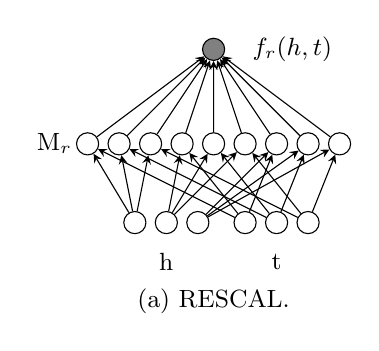
\begin{tikzpicture}[
        neuron/.style={circle, draw, fill=white, minimum size=8pt, inner sep=0pt},
        output/.style={circle, draw, fill=gray, minimum size=8pt, inner sep=0pt},
        connection/.style={-stealth, thin},
        label/.style={font=\small}
    ]
        % Input layer h (left)
        \foreach \i in {1,2,3} {
            \node[neuron] (h\i) at (\i*0.4 - 0.4, -1) {};
        }
        \node[label] at ([yshift=-0.5cm]h2) {h};
        
        % Input layer t (right)  
        \foreach \i in {1,2,3} {
            \node[neuron] (t\i) at (\i*0.4 + 1, -1) {};
        }
        \node[label] at ([yshift=-0.5cm]t2) {t};
        
        % Hidden layer Mr
        \foreach \i in {1,2,3,4,5,6,7,8,9} {
            \node[neuron] (mr\i) at (\i*0.4 - 1, 0) {};
        }
        \node[label] at ([xshift=-12pt]mr1) {M$_r$};
        
        % Output
        \node[output] (out1) at (1, 1.2) {};
        \node[label] at ([xshift=1cm]out1) {$f_r(h,t)$};
        
        % Connections from h to Mr
        \foreach \i in {1,2,3} {
            \foreach \j in {1,2,3} {
                \pgfmathtruncatemacro{\target}{(\i-1)*3+\j}
                \draw[connection] (h\i) -- (mr\target);
            }
        }
        
        % Connections from t to Mr
        \foreach \i in {1,2,3} {
            \foreach \j in {1, 2, 3} {
                \pgfmathtruncatemacro{\target}{\i + ((\j - 1) * 3)}
                \draw[connection] (t\i) -- (mr\target);
            }
        }
        
        % Connections from Mr to output
        \foreach \i in {1,2,3,4,5,6,7,8,9} {
            \draw[connection] (mr\i) -- (out1);
        }
        
        % Label
        \node[label] at (1, -2) {(a) RESCAL.};
    \end{tikzpicture}
    \hspace{1cm}
    % DistMult (b)
    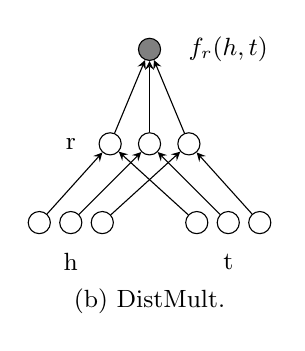
\begin{tikzpicture}[
        neuron/.style={circle, draw, fill=white, minimum size=8pt, inner sep=0pt},
        output/.style={circle, draw, fill=gray, minimum size=8pt, inner sep=0pt},
        connection/.style={-stealth, thin},
        label/.style={font=\small}
    ]
        % Input layer h (left)
        \node[label] (h_label) at (0, -1.5) {h};
        \foreach \i in {1,2,3} {
            \pgfmathsetmacro{\target}{(\i-2)*0.4}
            \node[neuron] (h2\i) at ([xshift=\target cm, yshift=0.5cm]h_label) {};
        }
        
        % Input layer t (right)
        \node[label] (t_label) at (2, -1.5) {t};
        \foreach \i in {1,2,3} {
            \pgfmathsetmacro{\target}{(\i-2)*0.4}
            \node[neuron] (t2\i) at ([xshift=\target cm, yshift=0.5cm]t_label) {};
        }
        
        % Hidden layer r
        \foreach \i in {1,2,3} {
            \node[neuron] (r2\i) at (0.5*\i, 0) {};
        }
        \node[label] at ([xshift=-0.5cm]r21) {r};
        
        % Output
        \node[output] (out2) at (1, 1.2) {};
        \node[label] at ([xshift=1cm]out2) {$f_r(h,t)$};
        
        % Connections - element-wise multiplication pattern
        \foreach \i in {1,2,3} {
            \draw[connection] (h2\i) -- (r2\i);
            \draw[connection] (t2\i) -- (r2\i);
            \draw[connection] (r2\i) -- (out2);
        }
        
        % Label
        \node[label] at (1, -2) {(b) DistMult.};
    \end{tikzpicture}
    \hspace{1cm}
    % HolE (c)
    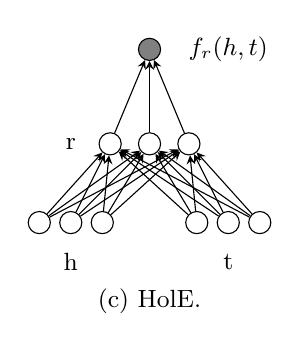
\begin{tikzpicture}[
        neuron/.style={circle, draw, fill=white, minimum size=8pt, inner sep=0pt},
        output/.style={circle, draw, fill=gray, minimum size=8pt, inner sep=0pt},
        connection/.style={-stealth, thin},
        label/.style={font=\small}
    ]
        % Input layer h (left)
        \node[label] (h_label) at (0, -1.5) {h};
        \foreach \i in {1,2,3} {
            \pgfmathsetmacro{\target}{(\i-2)*0.4}
            \node[neuron] (h3\i) at ([xshift=\target cm, yshift=0.5cm]h_label) {};
        }
        
        % Input layer t (right)
        \node[label] (t_label) at (2, -1.5) {t};
        \foreach \i in {1,2,3} {
            \pgfmathsetmacro{\target}{(\i-2)*0.4}
            \node[neuron] (t3\i) at ([xshift=\target cm, yshift=0.5cm]t_label) {};
        }
        
        % Hidden layer r
        \foreach \i in {1,2,3} {
            \node[neuron] (r3\i) at (0.5*\i, 0) {};
        }
        \node[label] at ([xshift=-0.5cm]r31) {r};
        
        % Output
        \node[output] (out3) at (1, 1.2) {};
        \node[label] at ([xshift=1cm]out3) {$f_r(h,t)$};
        
        % Connections - circular correlation pattern (more complex)
        \foreach \i in {1,2,3} {
            \foreach \j in {1,2,3} {
                \draw[connection] (h3\i) -- (r3\j);
                \draw[connection] (t3\i) -- (r3\j);
            }
        }
        
        % Connections from r to output
        \foreach \i in {1,2,3} {
            \draw[connection] (r3\i) -- (out3);
        }
        
        % Label
        \node[label] at (1, -2) {(c) HolE.};
    \end{tikzpicture}
    
    \caption{Simple illustrations of semantic matching models RESCAL, DistMult, and HolE \parencite{ZHANG2024123876}.}
    \label{fig:semantic_maching_models}
\end{figure}

\textbf{Semantic matching models} aim to learn embeddings that capture semantic compatibility between entities and relations, using neural architectures. These architectures assign high scores to semantically coherent triples $(h,r,t) \in \mathcal{F}$ and low scores to semantically false triples. To learn the semantics of entities and relations, a scoring function is used. Unlike translation distance models, the scoring function is maximized. To give practical examples, the thesis introduces three SMMs: $RESCAL$, $DistMult$ and $HolE$. Simple illustrations of these methods can be found in \autoref{fig:semantic_maching_models}.

$RESCAL$ uses a matrix $M_r$ for the embedding. The main benefit for this is that different dimensions of the head and tail entities are able to interact with each other. Because of this, $RESCAL$ is able to capture the relation distance \parencite{hogan2021knowledge}. With the head and tail entities $(h,t)$ and the relation matrix $M_r$, the scoring function is defined as $f_r(h,t) = h^T M_rt = \sum_{i = 0}^{d-1}\sum_{i = 0}^{d-1}[M_r]_{ij}\cdot[h]_i\cdot[t]_j$.

$DistMult$ improves slightly on time and space costs compared to $RESCAL$. This is achieved by only using the diagonal elements of $M_r$, $\text{diag}(M_r) = r$. Other than only using the diagonal values of matrix $M_r$, the scoring function is the same with $RESCAL$. It is defined as $f_r(h,t) = h^T \text{diag}(r)t = \sum_{i=0}^{d-1}[r]_i\cdot[h]_i\cdot[t]_i$ \parencite{hogan2021knowledge}.

$HolE$ uses a \textit{circular correlation operation} to combine the head and tail entities. The circular correlation operator is defined as $h\star t \in \mathbb{R}^d$, and in practise, it takes the sums along the diagonals of the outer product of two vectors. The circular correlation operator is used to capture edge direction \parencite{hogan2021knowledge}. With the circular correlation operation defined, the scoring function is defined as $f_r(h,t) = r^T(h \star t) = \sum_{l=0}^{d-1} [r]_l \sum_{k=0}^{d-1} [h]_k \cdot [t]_{(k+l)mod d}$.

\begin{table}[h]
\centering
\label{tab:kge_comparison}
\resizebox{\textwidth}{!}{%
\begin{tabular}{lllll}
\hline
\textbf{Method} & \textbf{Category} & \textbf{Entity Embedding} & \textbf{Relation Embedding} & \textbf{Loss Function} \\
\hline
TransE & TDM & $h, t \in \mathbb{R}^d$ & $r \in \mathbb{R}^d$ & $\|h + r - t\|_{1/2}$ \\
TransH & TDM & $h, t \in \mathbb{R}^d$ & $r, w_r \in \mathbb{R}^d$ & $\|(h - w_r^T hw_r) + r - (t - w_r^T tw_r)\|_2^2$ \\
TransR & TDM & $h, t \in \mathbb{R}^d$ & $r \in \mathbb{R}^k, M_r \in \mathbb{R}^{k \times d}$ & $\|M_r h + r - M_r t\|_2^2$ \\
RESCAL & SMM & $h, t \in \mathbb{R}^d$ & $M_r \in \mathbb{R}^{d \times d}$ & $h^T M_r t$ \\
DisMult & SMM & $h, t \in \mathbb{R}^d$ & $r \in \mathbb{R}^d$ & $h^T diag(r) t$ \\
HolE & SMM & $h, t \in \mathbb{R}^d$ & $r \in \mathbb{R}^d$ & $r^T (h \star t)$ \\
\hline
\end{tabular}%
}
\caption{Summary of KGE techniques. TDM stands for translation distance models and SMM for semantic matching models. Table from article \parencite{ZHANG2024123876}}
\end{table}


\subsection{Unified methods}
\label{subsec:unified_methods}

Similar to hybrid methods in \autoref{subsec:hybrid_method}, unified methods combine the strengths of embedding and path-based methods. In practise, unified methods use both meta-paths and they propagate the embedding space to create recommendations. Implementations are typically based on frameworks that combine graph neural networks and attention mechanisms \parencite{hogan2021knowledge}. The main idea behind GNNs is to enhance node representations with message propagation. This means that the information of the neighbouring nodes is encoded into a vector representation of the nodes of the graph. 

\newpage

\section{Recommendation with knowledge graphs}
\label{sec:KG-based_RS}

While the previous section discussed how knowledge graphs are modelled, this section will discuss how the models of KGs can be used to generate recommendations.

\subsection{Path-based KG recommender methods}

Path-based methods use meta-paths to create recommendations. These meta-paths connect two nodes together through a series of relations. A practical example is a movie recommender system: Let a movie domain KG have nodes for users ($U$), movies (item) ($I$) and directors ($D$). Then recommendation could be configured to mine meta-paths $UIDI$ and $UIUI$ for user-item-director-item or user-item-user-item paths. Using preconfigured meta-paths, the recommendations become more explainable. Different meta-paths are shown in \autoref{tab:movie_meta-paths}.

\begin{table}[h]
\centering
\caption{Examples of meta-paths in a movie recommender system. $U$ is user, $M$ is movie, $D$ is director and $G$ is genre.}
\label{tab:movie_meta-paths}
\begin{tabular}{lccc}
\toprule
Meta-path & Explanation \\
\midrule
$UMUM$        & "Movies that similar users like" \\
$UMDM$        & "Movies by director $D$" \\
$UMGM$        & "Movies in genre $G$" \\
$UMUMGM$      & "Movies in genres that similar users like" \\
\bottomrule
\end{tabular}
\end{table}

Among path-based approaches, \textit{Hete-MF} \parencite{Yu2013CollaborativeFW} and \textit{Hete-CF} \parencite{luo2014hete} are two early approaches. The Hete-MF approach derives $L$ distinct meta-paths to compute similarity measures between items within each pathway. This method incorporates item-based regularization into a weighted non-negative matrix factorization framework, enhancing the low-dimensional representations of both users and items. This then further improves the quality of recommendations. 

In contrast, Hete-CF determines user preferences for unrated items by incorporating multiple similarity components (user-user, item-item, and user-item relationships) as regularization constraints within its model. The superior performance of Hete-CF compared to Hete-MF is due to its comprehensive utilization of various similarity metrics in the recommendation process \parencite{guo2020survey}.


\subsection{Embedding-based KG recommender methods}
\label{subsec:embedding-based_methods_recommendation}

A KG embedding-based recommendation system generally consists of three parts: a KG, a graph embedding module, and a recommendation module \parencite{ZHANG2024123876}. The three components enable recommendation based on the data in the knowledge graph. The KG stores auxiliary information about items and users. The graph embedding module creates the embedding and the recommendation module uses the embedding to create recommendations. Then lastly, the recommendations are displayed to the user. 

To create recommendations based on graph embeddings, machine learning methods are used to analyse the embedding. This is typically modelled by a preference score $\hat{y}_{i,j} =  f(\textbf{u}_i, \textbf{v}_j)$ \parencite{ZHANG2024123876}, where the function $f: \mathbb{R}^d\times\mathbb{R}^d \rightarrow \mathbb{R}$, $\textbf{u}_i$ is the user latent vector and $\textbf{v}_j$ is the item latent vector. The function $f$ for calculating the preference score is typically a vector similarity calculation because the loss functions that create the embeddings group similar vectors together. Examples of vector similarity metrics are inner product and deep neural networks \parencite{ZHANG2024123876}. 

The scoring functions of embeddings can also be used for recommendation. If $d(\cdot, \cdot)$ is a distance function between two vectors, link predictions between users and items can be calculated by $d_{ij}(u_i + r, v_j)$. The smaller the distance, the more likely the relation $r$ is true in the original KG. This idea is visualized in \autoref{fig:link_prediction}. The figure shows an embedding of a movie KG, where true entity-relation-entity connections have a small error in the Euclidean distance between the entities. 

\begin{figure}[h]
    \centering
    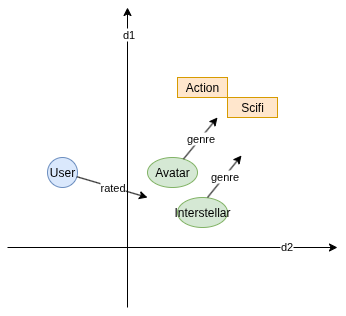
\includegraphics[width=0.5\linewidth]{images/embedding_example.png}
    \caption{A 2-dimensional translation distance embedding. Avatar and Interstellar are likely similar movies because they are close to each other. The user is likely to like both of the movies.}
    \label{fig:link_prediction}
\end{figure}

\subsection{Unified KG recommender methods}

Unified methods mainly consist of graph neural networks \parencite{hogan2021knowledge} and these methods use message passing (path propagation) to improve node embeddings in the KG. The node embedding vectors will contain the semantic information of the node and its neighbours, so the embedded node representations can be processed with machine learning. The machine learning done to the embedded vectors is similar to the methods introduced in \autoref{subsec:embedding-based_methods_recommendation}.

\subsection{Advantages of knowledge graph enhanced recommender systems}

Compared to traditional recommender systems, KG-based systems have \textit{better representation of data} \parencite{jetti2025knowledge}. This is because traditional recommender systems base recommendations only on user-item interaction data. KG-based systems also incorporate auxiliary information about users and items. This information can be user-side or items-side information. User-side auxiliary information could be user age, address, occupation and gender. Examples of item-side auxiliary information are brand, category and price. 

Another advantage of integrating KGs into a RS is that KG-based recommendations are \textit{more explainable} than traditional recommender systems. This is especially evident in path-based methods where recommendations are based on the connections between users and items in the KG. When recommendations are explainable, the RS is more trustable and transparent and it is easier for the user to understand what data is being collected from them and where it is being used.

\subsection{Limitations of knowledge graph enhanced recommender systems}

Constructing and integrating a KG into a recommender system is challenging. First, a knowledge graph has to be acquired. There are two main ways to do this: The first is to create a custom graph only used for a specific domain. Creating a custom graph requires a system that can gather data and store it in graph form. The second approach is to use an open source graph that is readily available on the internet. For integrating an open source graph into the RS, there are challenges in mapping the nodes in the KG to nodes in the RS. The mapping process typically introduces biases to the KG because of items having different names in the RS than in the KG or synonyms and homonyms.

The way a KG is constructed can introduce biases. The paper by \textcite{voit2021biasknowledgegraphs} found that knowledge graphs deliver different recommendations based on the language version of the graph. In the article they used different language versions of DBpedia, which is a KG constructed from Wikipedia data. For example, the article found that recommendations based on the English KG version were more likely to recommend English movies. 

Compared to traditional recommender systems, adding a KG recommendation module will increase computational costs, memory requirements and system complexity \parencite{jetti2025knowledge}. Higher computational and memory requirements might hinder scalability, and an increase in system complexity makes maintaining it more laborious. 


\subsection{Open source knowledge graphs}
\label{subsec:open_source_KG}

Knowledge graphs can be divided into two categories based on their scope: cross-domain KGs and domain-specific KGs \parencite{guo2020survey}. Cross-domain KGs are typically found in application scenarios that contain cross-disciplinary information. An example of a cross-domain RS is a search engine. Examples of cross-domain knowledge graphs are \textit{freebase}, \textit{Wikidata}, and \textit{DBpedia}. A popular domain-specific data set is \textit{Bio2RDF} \parencite{guo2020survey}. They provide linked data for life sciences. 

\begin{table}[h]
\centering
\label{tab:knowledge_datasets}
\begin{tabular}{lccc}
\toprule
Dataset & Website \\
\midrule
DBpedia     & \url{https://www.dbpedia.org/resources/knowledge-graphs/} \\
Freebase    & \url{https://developers.google.com/freebase/} \\
Wikidata    & \url{https://www.wikidata.org/wiki/} \\
Bio2RDF     & \url{https://download.bio2rdf.org/files/release/3/release.html} \\
\bottomrule
\end{tabular}
\caption{Datasets with general knowledge when originally released. Table inspired by article \parencite{ji2021survey}.}
\end{table}

\newpage

\section{Conclusions}

Knowledge graph-based recommender systems solve data sparsity issues and are more explainable than traditional recommender systems. The disadvantages of knowledge graph-based recommender systems are that the graphs are difficult to construct and that they increase model complexity and computational requirements. In practise, the most performative recommender systems are constructed by combining multiple different methods that use different aspects of the data. 


\section{Summary}

The thesis investigated how knowledge graphs can benefit recommender systems. This was done by first reviewing different types of recommender systems. The three types were content-based, collaborative and hybrid filtering. Content-based filtering detects similar items by comparing latent vectors of the items. Collaborative filtering creates recommendations based on collaborative data between users and items. Unified methods combine the strengths of different methods to create more performant methods.

Knowledge graphs can be used as auxiliary information in recommender systems. Methods for modelling knowledge graphs in recommender systems are path-based, embedding-based and unified methods. Path-based methods create recommendations based on paths in the knowledge graph. Embedding-based methods embed the knowledge graph into a low-dimensional space and unified methods combine the strengths of both path-based and embedding-based methods to create more accurate recommender systems.

Knowledge graph-based recommender systems solve data sparsity and explainability issues. They do this by using auxiliary information, in addition to user-item interaction data. Knowledge graphs can be created from scratch, or one can use free open-source graphs. Path-based methods especially create human understandable recommendations utilizing meta-paths. Embedding-based methods are able to encode the graph information as vectors so that machine learning methods can be used to create recommendations.

\section{Future directions}

A big problem of KGs is that they are expensive to generate. A proposed method for automatically generating KGs is \textit{word embedding techniques} used in large language models to learn the semantic meanings of words \parencite{hogan2021knowledge}. Word embedding techniques take sentences as input and create vector embeddings based on the semantic similarities of words in the given input text. For example, the words subway and metro would be assigned similar embedding vectors because they appear in similar contexts. Additionally, words with similar relationships, such as king and queen and husband and wife, will have similar relation embeddings. A popular method for embedding words is word2vec \parencite{mikolov2013efficient}.

Because constructing knowledge graphs is expensive, so is updating and maintaining them. All large-scale open-source KGs are static graphs, which means they do not update their information online. This means that static KGs are biased towards older items because they are more connected in the graph. \textit{Introducing dynamicity} would remove these biases. Applying dynamic knowledge graphs to recommender systems would help remove time-dependent biases. 

Article \parencite{zhang2024does} questions the need for all relations in the KG. The article does this by comparing the performance of recommender systems in three cases. The first case is the default case with the original KG. The second case is with false knowledge in the knowledge graph. False knowledge, in their study, means incorrect relations. The third case is with decreasing knowledge, meaning that some relations in the graph were deleted. Then these three states of the knowledge graph were benchmarked in both the cold-start and the default case. 

The researchers found that decreasing authentic knowledge in the KG does not significantly reduce the performance of the recommender system. This could be caused by noisy knowledge graph information. The KGs used in the study were large open source KGs and were not optimized for the recommendation task at hand. \textit{Knowledge graph pruning} could be used to reduce the amount of redundant relations in the graph to save both compute time and memory requirements.  


\clearpage

\printbibliography

\end{document}


